\documentclass{scrartcl}
\usepackage{mm_ws15}

\newcommand{\sheetTitle}{Blatt 4, Abgabe 17.11.2015 12:00}
\begin{document}
\maketitle


\section{Das Methanmolekül \points{6}}
Ein Methanmolekül (chemische Formel $\mathrm{CH}_4$) besitzt die Struktur eines regulären Tetraheders (siehe Bild).
Die Wasserstoffatome (weiß) befinden sich dabei in den Punkten $(0,0,0)$, $(k,k,0)$, $(k,0,k)$ und $(0,k,k)$; das Kohlenstoff im Zentrum im Punkt $(\frac{k}{2},\frac{k}{2},\frac{k}{2})$.
Hierbei bezeichnet $k$ eine Längenkonstante.
\begin{subex}
  \item Zeigen Sie, dass die angegebene Struktur tatsächlich einen regulären Tetraeder bilden, d.h.\ dass alle Verbindungslinien zwischen den Wasserstoffatomen gleich lang sind.
  \item Berechnen Sie den Bindungswinkel zwischen zwei Wasserstoffatomen, d.h.\ den Winkel, der von zwei Wasserstoffatomen mit dem Kohlenstoffatom im Scheitelpunkt aufgespannt wird.
\end{subex}

\begin{center}
  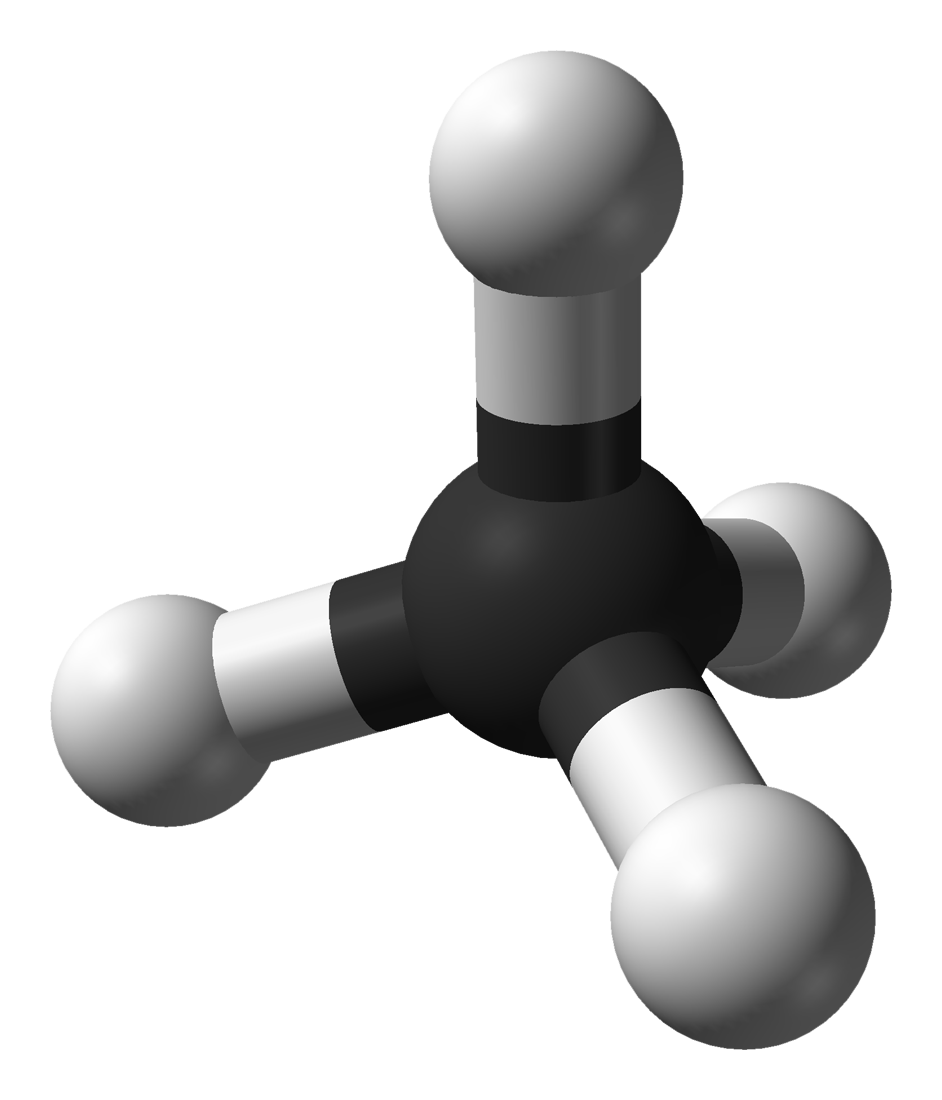
\includegraphics[width=3cm]{img/methan.png}
\end{center}


\section{Eigenschaften des Vektorproduktes \points{6}}
In dieser Aufgabe sollen Sie die folgenden Eigenschaften des Vektorproduktes nachweisen:
Für drei Vektoren $\vec{u},\vec{v},\vec{w} \in \RR^3$ gilt
\begin{itemize}
  \item $\vec{u} \times \vec{v} = - \vec{v} \times \vec{u}$ (Antikommutativität)
  \item $(\vec{u} \times \vec{v}) \times \vec{w} \neq \vec{u} \times (\vec{v} \times \vec{w})$ (keine Assoziativität)
  \item $\sp{\vec{u}}{\vec{v} \times \vec{w}} = \sp{\vec{w}}{ \vec{u} \times \vec{v}} = \sp{\vec{v}}{ \vec{w} \times \vec{u}}$ (zyklische Vertauschbarkeit)
\end{itemize}
Hier bezeichnet $\sp{\cdot}{\cdot}$ das euklidische Skalarprodukt.

\begin{remark}{Hinweis}
  Sie können diese Beziehungen in Komponentenschreibweise der Vektoren zeigen, was aber viel aufwendige Schreibarbeit bedeutet.
  Alternativ können Sie aber auch die Definition über das  so genannten \emph{Levi-Civita-Symbols} $\epsilon_{ijk}$ verwenden.
  Für die $i$-te Komponente des Kreuzproduktes gilt
  \[
    (\vec{u}\times \vec{v})_i = \sum_{j,k =1}^3 \epsilon_{ijk}\, u_j\,v_k
  \]
  mit
  \begin{gather}
    \epsilon_{ijk} =
    \begin{cases}
      +1 &\textrm{falls}\ (i,j,k)\ \textrm{zyklische Permutation von } (1,2,3)\\
      -1 &\textrm{falls}\ (i,j,k)\ \textrm{azyklische Permutation von } (1,2,3)\\
      0 &\textrm{sonst}
    \end{cases}
    \nonumber
  \end{gather}
  Eine Permutation von $n$ Elementen $\sigma$ (siehe auch Blatt 1) heißt \emph{zyklisch}, wenn sie alle Elemente um die gleiche Zahl von Stellen verschiebt, d.h.
  \[
    \sigma(i) = i \oplus k = \operatorname{mod}_n(i + k)
  \]
  für ein $k \in \NN$ (siehe auch Übungsblatt 1).
  Wenn eine Permutation nicht zyklisch ist, heißt sie azyklisch.
  Machen Sie sich klar, dass $\epsilon_{123}=\epsilon_{231}=\epsilon_{312}=1$, $\epsilon_{132}=\epsilon_{321}=\epsilon_{213}=-1$ und $0$ in allen anderen Fällen.
\end{remark}


\section{Vektorprodukte \points{6}} 
Berechnen Sie die folgenden Vektorprodukte.
Prüfen Sie jeweils auch explizit, ob $\vec{a} \times \vec{b}$ senkrecht auf $\vec{a}$ und $\vec{b}$ steht.

\begin{subex*}
  \item $\colvec{1 \\ 2 \\ 3} \times \colvec{4 \\ 5 \\ 6}$
  \item $\colvec{\sqrt{2} \\ \sqrt{8} \\ 1} \times \colvec{1 \\ 2 \\ \frac{\sqrt{2}}{2}}$
  \item $\colvec{\frac{1}{\sqrt{2}} \\ \frac{1}{\sqrt{2}} \\ 0} \times \colvec{\frac{1}{\sqrt{2}} \\ 0 \\ -\frac{1}{\sqrt{2}}}$
\end{subex*}

\section{Grenzwerte reeller Funktionen \points{12}}
In der Vorlesung haben Sie die den Grenzwert einer reellen Funktion $f\colon \RR \to \RR$ kennen gelernt:
$y \in \RR$ heißt Grenzwert von $f$ an der Stelle $x_0 \in \RR$, wenn für alle $\epsilon > 0$ ein $\delta > 0$ exisiert, sodass für alle $x \in \RR$ mit $\abs{x - x_0} < \delta$ gilt $\abs{f(x) - y} < \epsilon$.
Man schreibt für den Grenzwert dann $y = \lim_{x \to x_0} f(x)$.

Analog definiert man den Grenzwert für \quotes{$x_0 = \pm\infty$}: 
$y = \lim_{x \to \infty}$ ($y = \lim_{x \to -\infty}$) wenn für alle $\epsilon > 0$ ein $S \in \RR$ exisiert, sodass für $x > S$ ($x < S$) folgt $\abs{f(x) - y} < \epsilon$. 

\begin{subex}
  \item\points{5} Beweisen Sie, dass $\lim_{x \to -3} 1 - 4x = 13$ (mit anderen Worten: für gegebens $\epsilon$, bestimmen Sie $\delta$).
  Was ist der Grenzwert $\lim_{x \to 3} 1 - 4x$?
  Beweisen Sie das!
  \item\points{4} Betrachte $f(x) = \frac{1}{2^x}$.
  Skizzieren Sie den Verlauf der Funktion für $x \in \RR$.
  Was passiert für große $x$; was passiert für kleine $x$?
  Mit anderen Worten: Geben Sie den Grenzwert von $f$ für $x \to \infty$ und $x \to -\infty$ an.
  Bestimmen Sie außerdem $\lim_{x \to 0} f(x)$.
  \item\points{3} Existieren die folgenden Grenzwerte? 
  Wenn ja, geben Sie diese an.
  Begründen Sie Ihr Ergebnis kurz (kein Beweis!).
  \[
    \lim_{x \to 0} x \, \sin \left( \frac{1}{x} \right)  \quad\quad
    \lim_{x \to \infty} \sin x  \quad\quad 
    \lim_{x \to -2} \frac{x^2 - 4}{x + 2}
  \]
\end{subex}

\end{document}